\section{Durchführung}
\label{sec:Durchführung}

Der Aufbau der Schaltungen erfolgt auf einer Steckplatine (Breadboard), wobei der OPV über ein Netzgerät mit einer symmetrischen Betriebsspannung von $U_S = \pm 15\,\text{V}$ versorgt wird. Zur Signalerzeugung wird ein Funktionsgenerator verwendet. Zur Analyse der Ein- und Ausgangssignale wird ein digitales Speicheroszilloskop eingesetzt. Dort können Spannungsamplituden direkt abgelesen und die Ausschnitte der Spannungskurven als PDF exportiert werden. Ein beispielhafter Aufbau, wie er hier für den Linearverstärker genutzt wurde, ist in \autoref{fig:100} zu sehen. Das Speicheroszilloskop ist in \autoref{fig:101} abgebildet. 

\begin{figure}[H]
     \centering
     \begin{subfigure}[b]{0.45\textwidth}
         \centering
         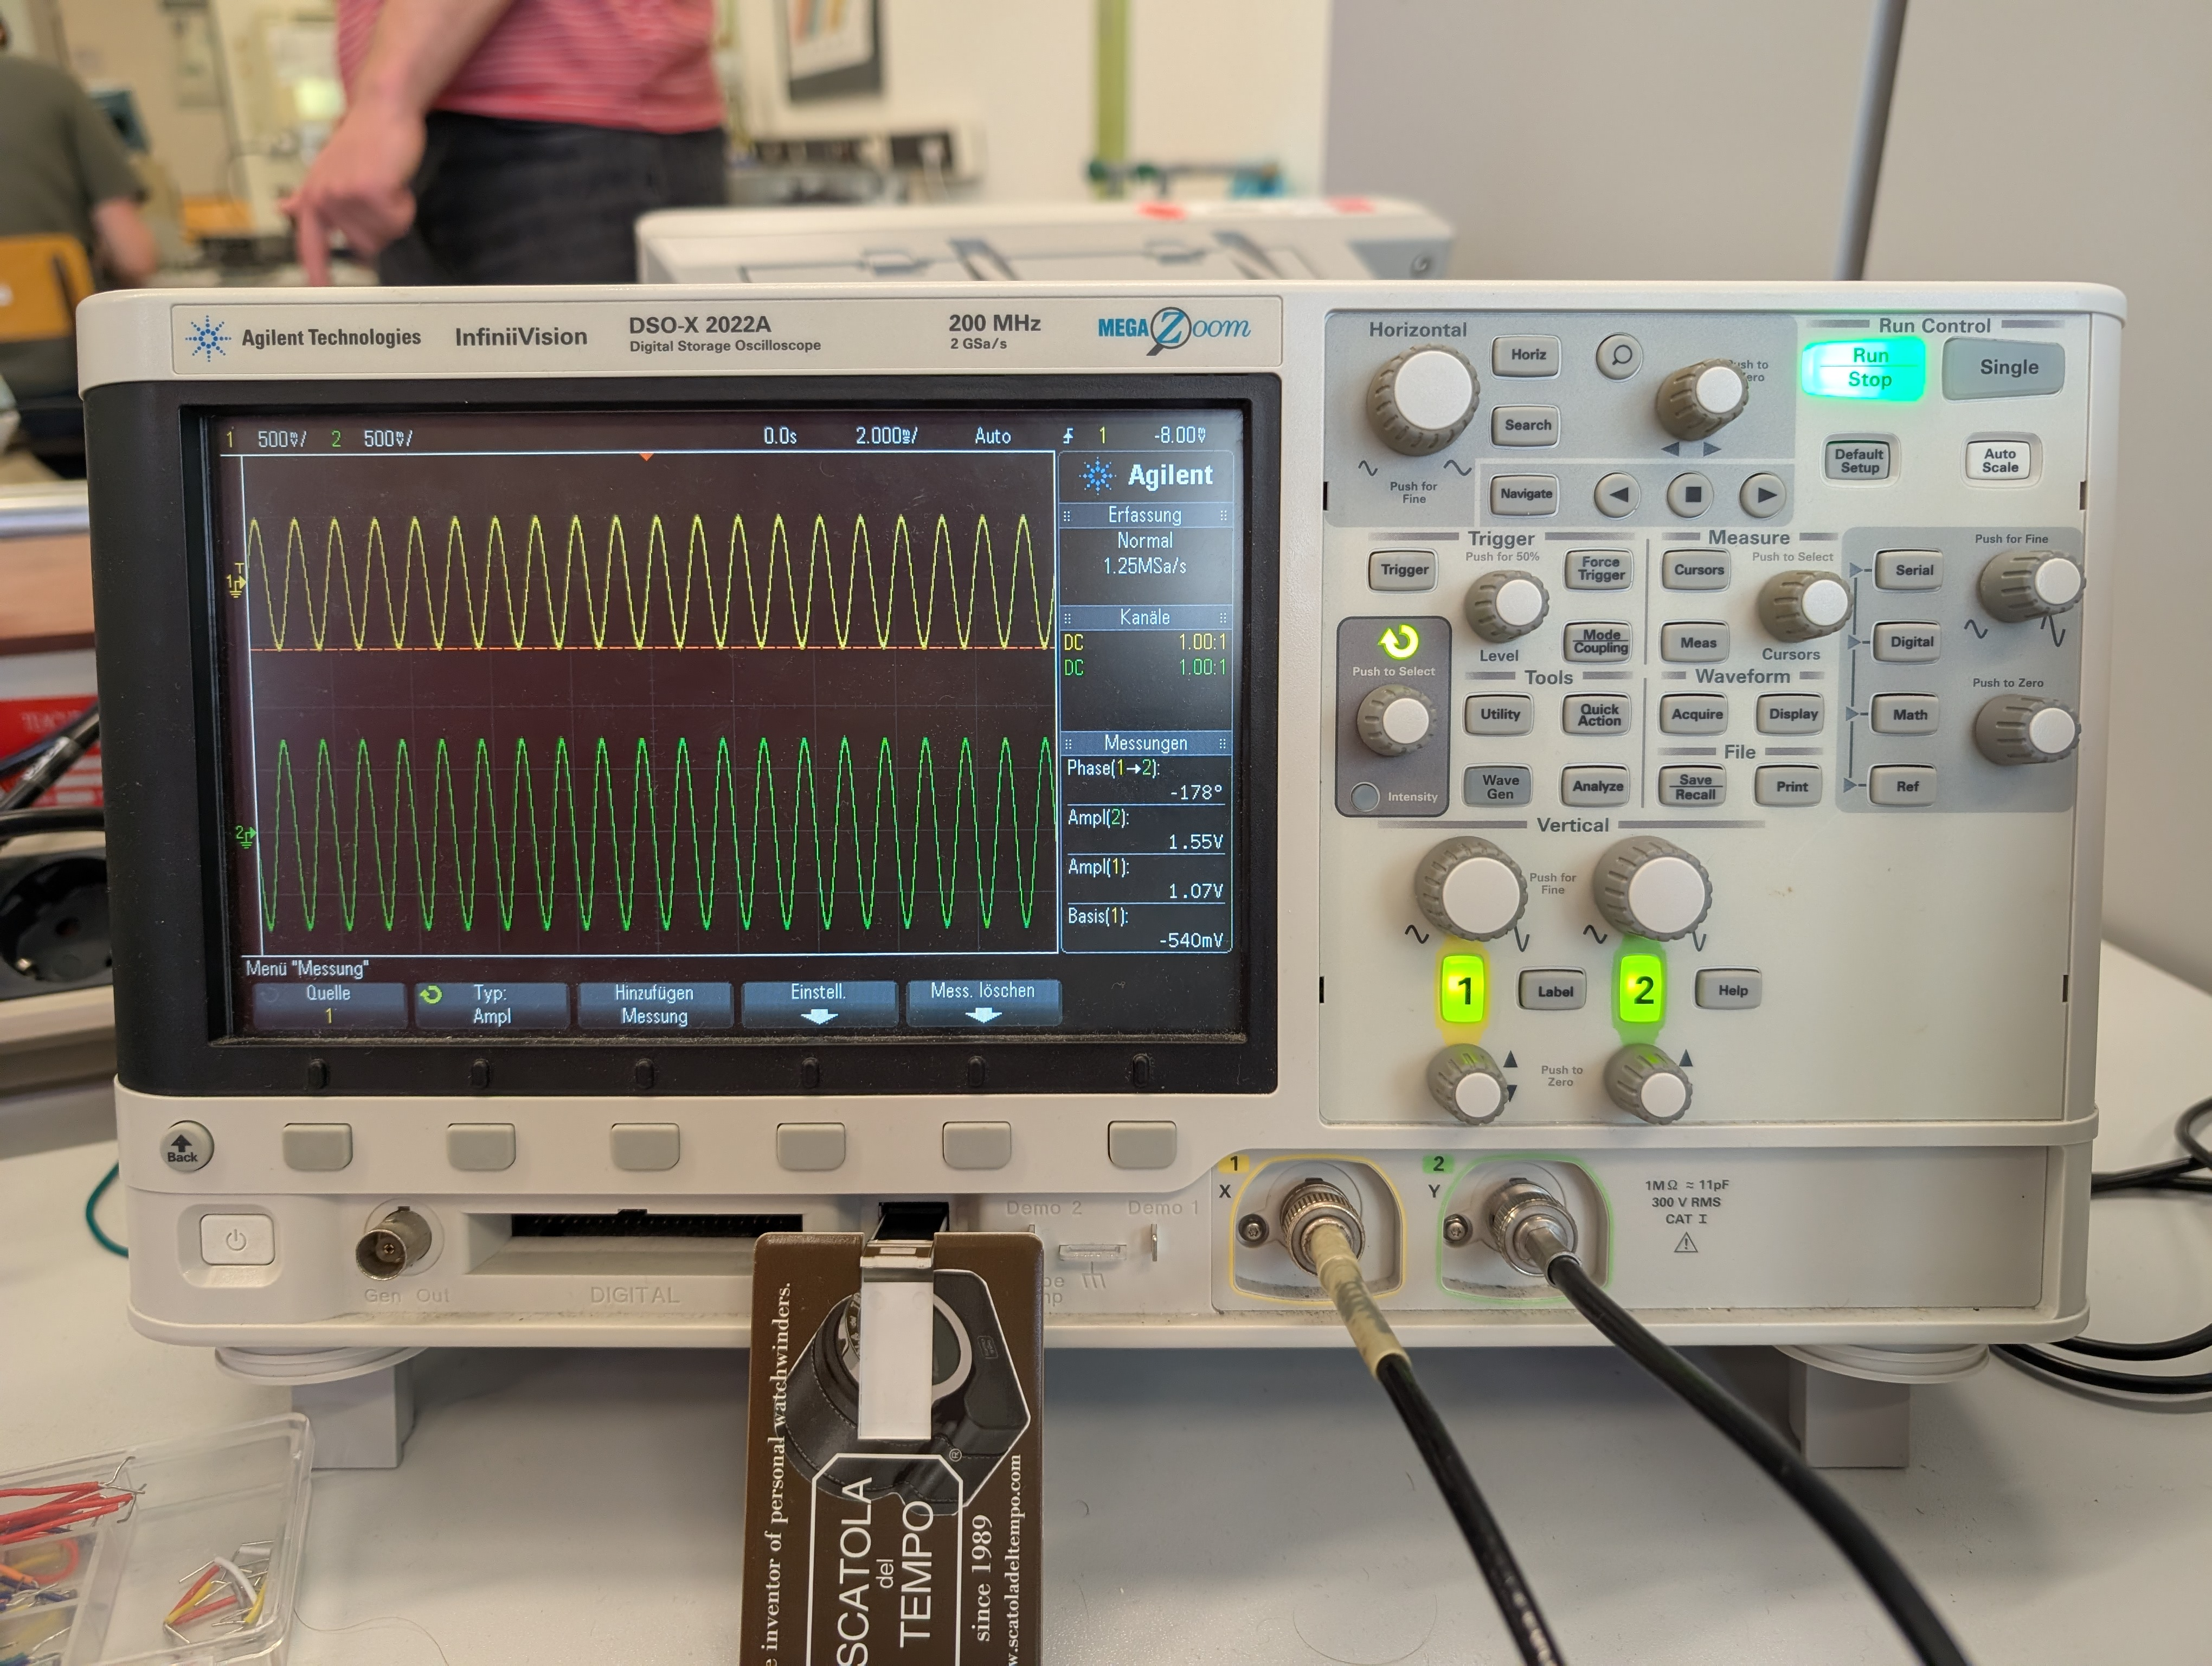
\includegraphics[width=\textwidth]{Bilder/1000040074.jpg}
         \caption{Digitales Speicheroszilloskop}
         \label{fig:101}
     \end{subfigure}
     \hfill
     \begin{subfigure}[b]{0.45\textwidth}
         \centering
         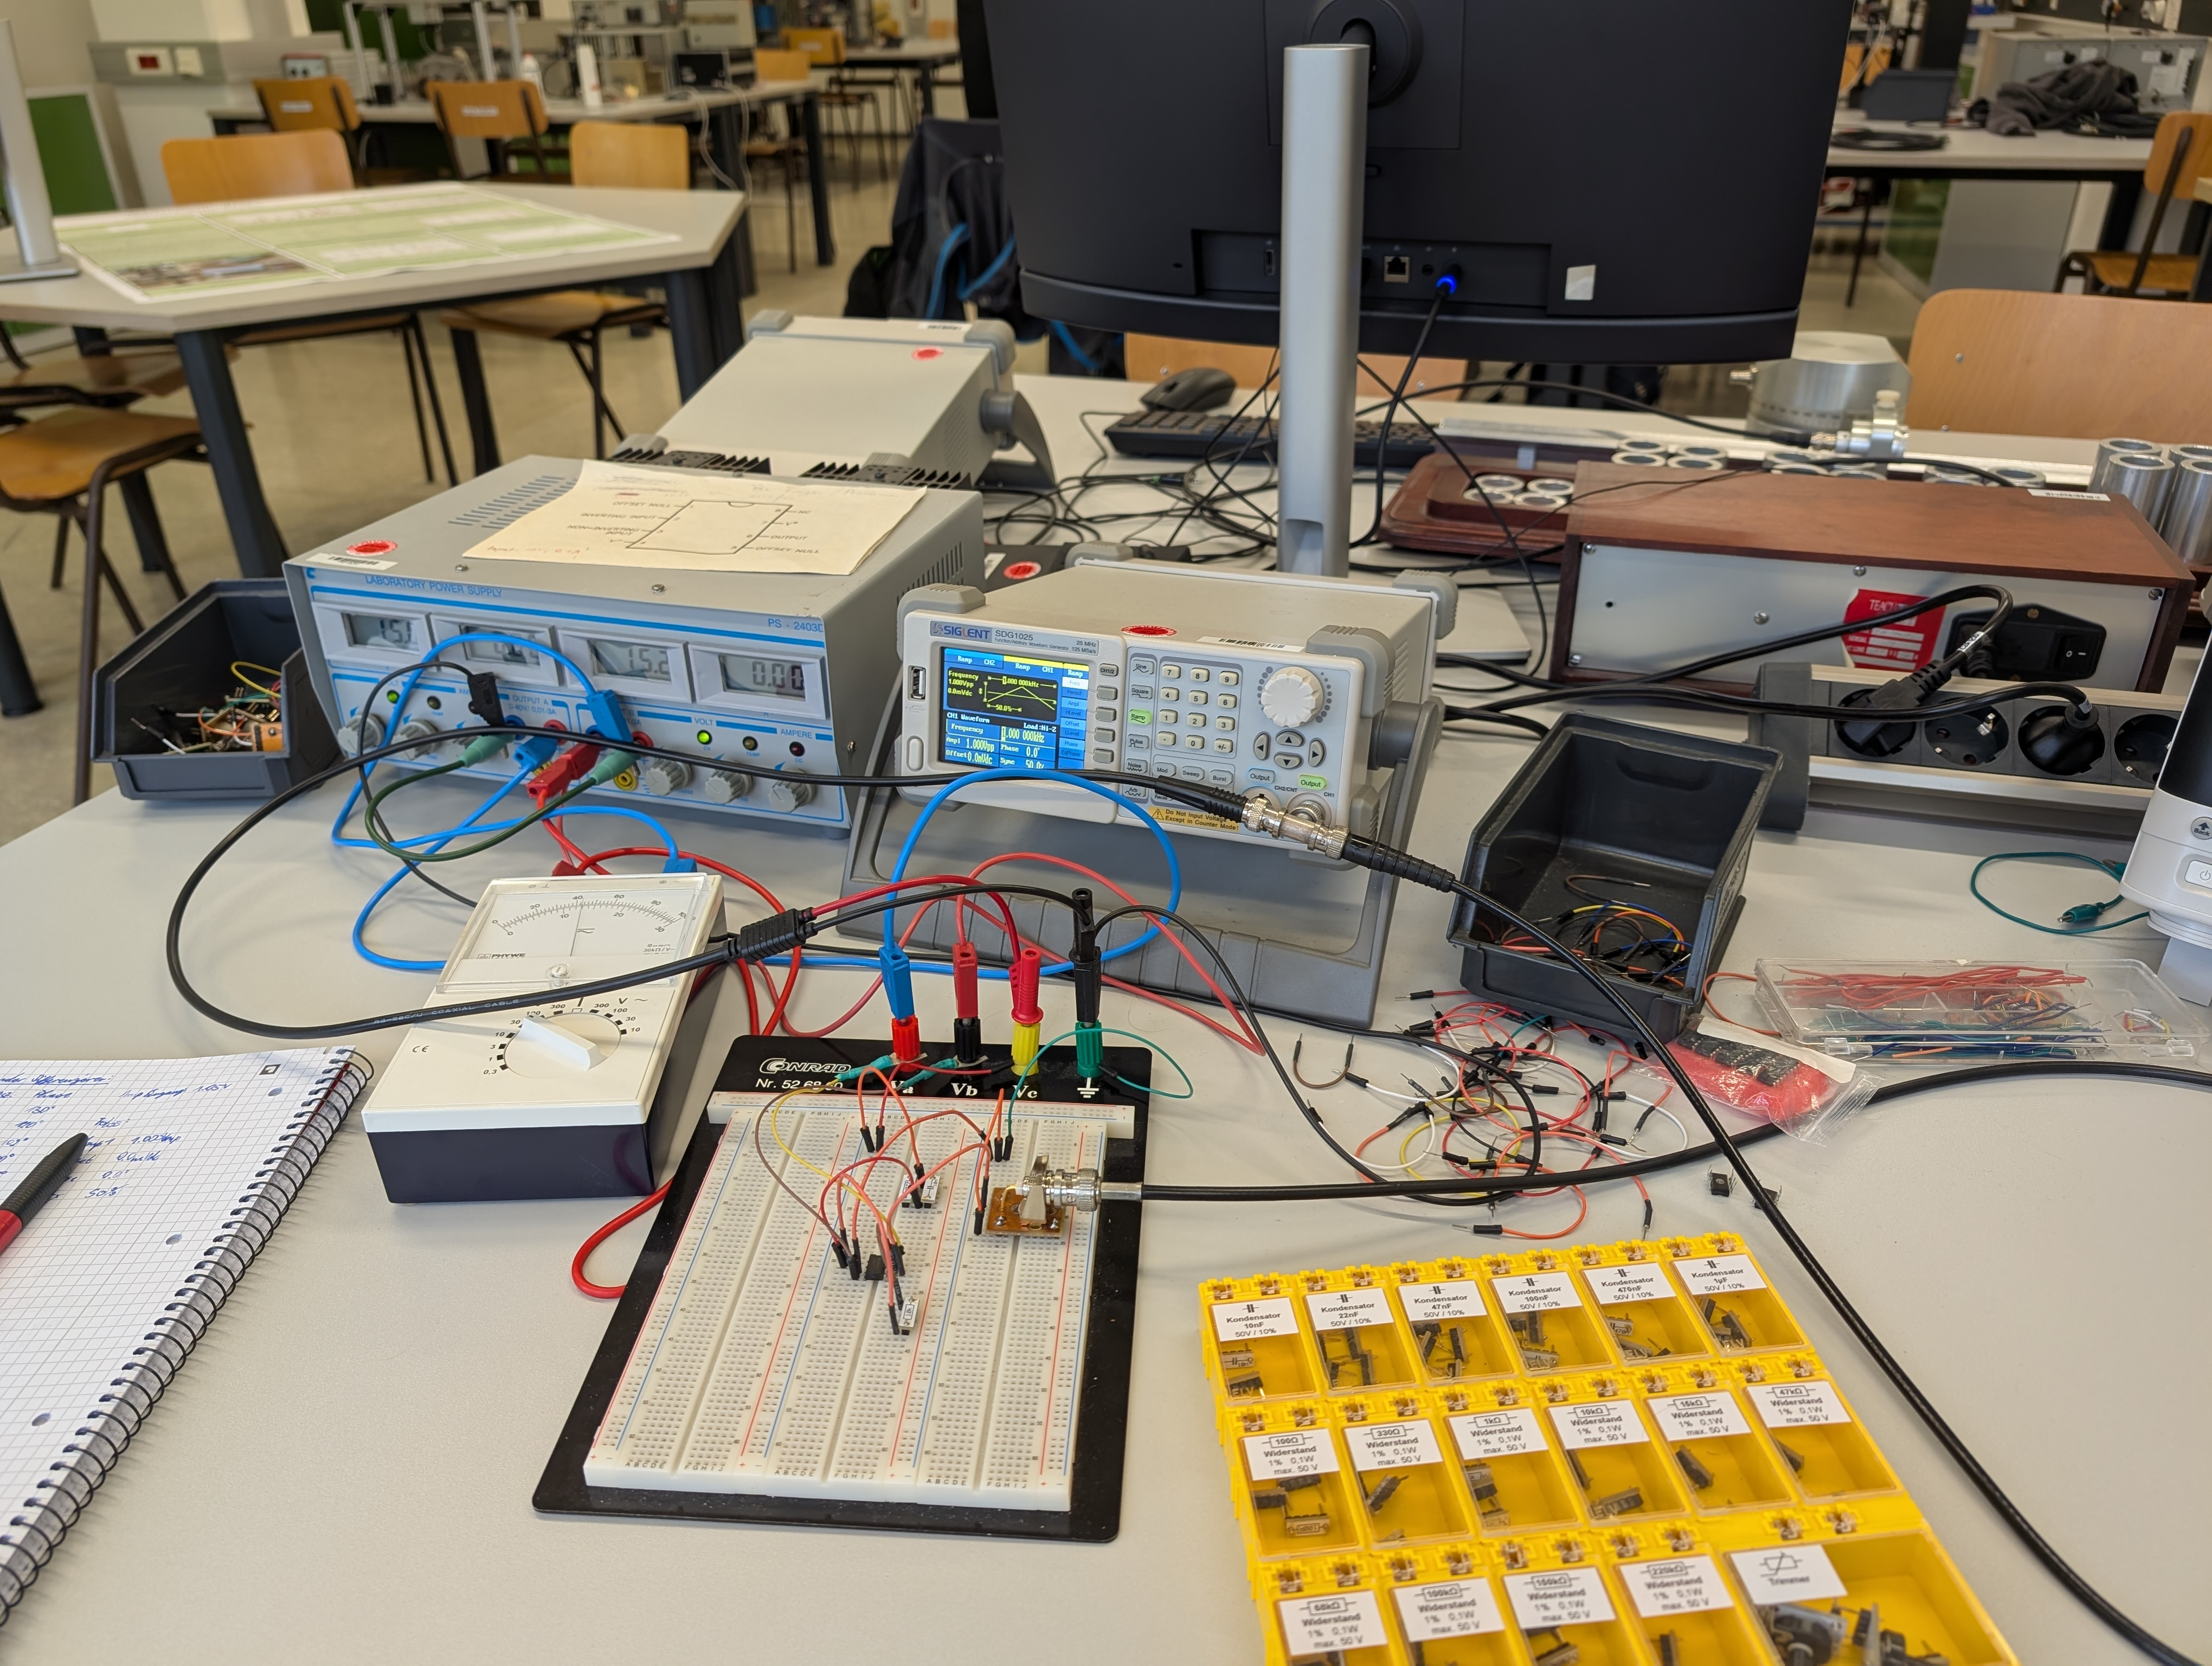
\includegraphics[width=\textwidth]{Bilder/1000040084.jpg}
         \caption{Aufbau des invertierenden Linearverstärkers}
         \label{fig:100}
     \end{subfigure}
     \caption{Messplatz und beispielhafter Schaltungsaufbau.}
\end{figure}

\subsection{Invertierender Linearverstärker}

In \autoref{fig:102} ist der Schaltplan für den invertierenden Linearverstärker zu sehen. Danach wird die Schaltung aufgebaut und es wird mit vier unterschiedlichen Widerstandsverhältnissen, also vier Verstärkungsgraden,
\begin{align}
    \frac{R_2}{R_1} &= 1{,}5 &
    \frac{R_2}{R_1} &= 10 &
    \frac{R_2}{R_1} &= 4{,}7 &
    \frac{R_2}{R_1} &= 3{,}1
\end{align}
sowie einer Eingangsamplitude von $\qty{1.05}{\volt}$ die Frequenzabhängigkeit der Ausgangsspannung des Verstärkers untersucht. Dabei wird der Frequenzpunkt gesucht, an dem die Ausgangsspannung abfällt.

\begin{figure}[H]
    \centering
    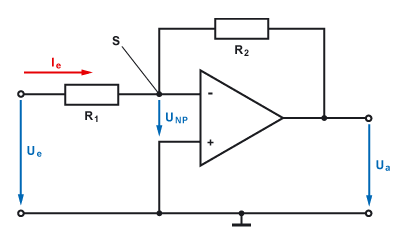
\includegraphics[width=0.7\textwidth]{Bilder/Screenshot_20260511_130927.png}
    \caption{Schaltung des invertierenden Linearverstärkers \cite{projektlabor_invertierend}.}
    \label{fig:102}
\end{figure}

\subsection{Umkehr-Integrator und invertierender Differenzierer}
Für den Integrierer und Differenzierer wird bis auf einen Unterschied das Schaltbild aus \autoref{fig:102} verwendet. Beim Integrierer wird der Widerstand $R_2$ durch eine Kapazität $C$ ersetzt. Beim Differenzierer wird the Widerstand $R_1$ durch die Kapazität ersetzt. Hierbei soll die Funktion der Schaltung als Integrierer bzw. Differenzierer verifiziert werden. Dazu werden als Signalspannungen jeweils eine Dreiecks-, Rechtecks- und Sinusspannung angelegt und das Ausgangssignal auf dem Oszilloskop exportiert. 

Die Messungen werden bei einer Eingangsspannung von $\qty{1.05}{\volt}$ sowie einer Frequenz von $f = \qty{1e6}{Hz}$ aufgenommen.

Die Schaltungen für den Integrierer sowie den Differenzierer sind in \autoref{fig:105} zu sehen.

\begin{figure}[H]
     \centering
     \begin{subfigure}[b]{0.45\textwidth}
         \centering
         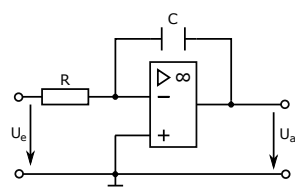
\includegraphics[width=\textwidth]{Bilder/integrator.png}
         \caption{Schaltplan zum Integrierer mit der rückgekoppelten Kapazität}
         \label{fig:bild1}
     \end{subfigure}
     \hfill
     \begin{subfigure}[b]{0.45\textwidth}
         \centering
         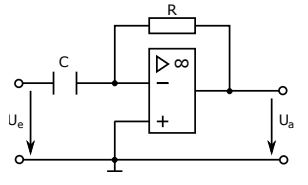
\includegraphics[width=\textwidth]{Bilder/Differenzierer.png}
         \caption{Schaltplan zum Differenzierer mit der Kapazität am Eingang}
         \label{fig:bild2}
     \end{subfigure}
     \caption{Schaltpläne der zeitabhängigen OPV-Grundschaltungen.}
     \label{fig:105}
\end{figure}

\subsection{Nicht-invertierender Schmitt-Trigger}
Es soll die Hysteresekurve der nicht-invertierenden Schmitt-Trigger-Schaltung aufgenommen werden. Dazu wird die Schaltung aufgebaut und anschließend die Eingangsspannung so lange von Null an ins Positive variiert, bis die Ausgangsspannung in die Sättigung fällt, also die obere Kippspannung erreicht wurde. Analog wird für die negative Kippspannung verfahren. 

Daraus lässt sich die experimentelle Hysteresekurve mit positiver und negativer Kippspannung konstruieren. Die theoretischen Grenzspannungen lassen sich über das Widerstandsverhältnis gemäß der Formel $U_{\text{kipp}} = \pm U_S \cdot \frac{R_1}{R_1+R_2}$ bestimmen (die explizite Berechnung und der Vergleich mit den Messwerten erfolgt im entsprechenden Kapitel der Auswertung).

\begin{figure}[H]
    \centering
    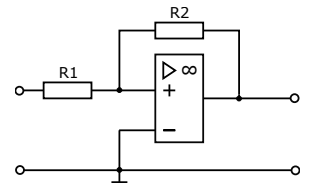
\includegraphics[width=0.6\textwidth]{Bilder/Schmidt.png}
    \caption{Schaltplan des nicht-invertierenden Schmitt-Triggers.}
    \label{fig:schmitt_schaltung}
\end{figure}